\chapter{Lecture: Heaps and Heap Sort}
\href{https://ocw.mit.edu/courses/electrical-engineering-and-computer-science/6-006-introduction-to-algorithms-fall-2011/lecture-videos/lecture-4-heaps-and-heap-sort/}{Lecture 4} from the MIT's 
Intro to Algorithms.

We will use heap as an example of an implementation of a priority queue.
\begin{definition}
	Priority Queue implements a set \(S\) of elements, each of the elements is associated
	with a key.
\end{definition}
\noindent
A heap is classified as an Abstract Data Type (ADT). We will specify the set of operations we would like
to perform on a priority queue?
\begin{enumerate}[label=$\ast$]
	\item Insert \((S, x)\): insert \(x\) into a set of \(S\)
	\item \(\max (S)\): return the element of \(S\) with the largest key
	\item extract-\(\max(S)\): and remove from \(S\)
	\item increase priority key \((S, x, k)\): increase the value of \(x\)'s key to \(k\).
\end{enumerate}
A heap is an implementation of a priority queue. An array visualized as a nearly complete binary
tree.
\begin{figure}[h]
	\centering
	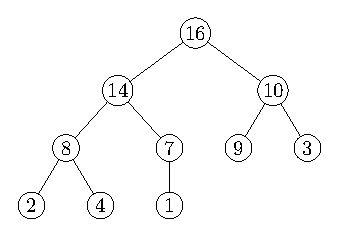
\includegraphics[width=3in]{binary_tree_lec4.pdf}
	\caption{Binary Tree: follows the max heap property.}
	\label{fig4:binary_search_tree}
\end{figure}
With a heap as a tree, the root element is the first element with \(i = 1\), parent\((i) = i / 2\), left\((i) = 2\), 
and right\((i) = 2i + 1\). The max heap property says that the key of a node is greater than or equal to
the keys of its children. For min heap, replace \(\geq\) with \(\leq\). How do we build a max heap out of 
an initially unsorted array? Heap operations:
\begin{enumerate}[label=$\ast$]
	\item build\_max\_heap: produces a max heap from an arbitrary array.
	\item max\_heapify: correct a single violation of the heap property in a sub-tree's root.
\end{enumerate}
For max\_heapify\((A, i)\), we assume that the tree's rooted at left\((i)\) and right\((i)\) are max heaps.
\begin{figure}[h]
	\centering
	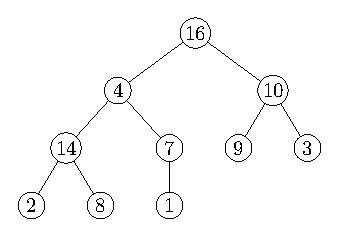
\includegraphics[width=3in]{max_heapify_example_lec4.pdf}
	\caption{Consider this binary representation for a heap. We need to max\_heapify this tree.}
	\label{fig4:max_heapify}
\end{figure}
For \cref{fig4:max_heapify}, we call max\_heapify\((A, 2)\). What does this code do?
\begin{enumerate}[label=$\ast$]
	\item Exchange \(A[2]\) with \(A[4]\)
	\item Call max\_heapify\(A[4]\)
	\item Exchange \(A[9]\) with \(A[4]\)
\end{enumerate}
The complexity of max\_heapify would be \(\theta(\log_2 n)\). How would we use max\_heapify to 
create build\_max\_heap? To convert \(A[a,\ldots, n]\) into a max heap, What is the complexity of build?
\(O(n\log_2 n)\), can we do better than this (simple analysis)?
Through careful analysis, we have \(\theta(n)\) complexity. Observe that max\_heapify takes constant
time \(O(1)\) for nodes that are one level above leaves, and in general, \(O(\ell)\) time for nodes that
are \(\ell\) levels above the leaves. We have \(n / 4\) nodes with level \(1\), \(n / 8\) with level \(2\), ... and
\(1\) node level \(\log_2 n\). The total amount of work in the for loop can be summed as
\[
	\frac{n}{4}\cdot c + \frac{n}{8}\cdot 2c + \frac{n}{16}\cdot 3c + \cdots + 1\cdot\log_2 n\cdot c
\]
Set \(n / 4 = 2^k\) then we have 
\[
	c\cdot 2^k \Big(\frac{1}{2^0} + \frac{2}{2^1} + \frac{3}{2^2} + \cdots + \frac{k + 1}{2^k}\Big)
	= c\cdot 2^k\cdot\sum_{i = 0}^k\frac{i + 1}{2^i}\leq M
\]
where \(M\) is a constant. Thus, we have \(\theta(c\cdot n /4 \cdot M) \rightarrow \theta(n)\) complexity.
\begin{enumerate}
	\item Build max heap from unsorted array; \(\theta(n)\)
	\item Find max element \(A[1]\)
	\item Swap elements \(A[n]\) with \(A[1]\); now the max element is at the end of the array
	\item Discard node \(n\) from the heap simply by decrementing the heap size.
	\item New root after the swap may violate the max heap property but the children are max heaps
	\item Run max\_heapify
\end{enumerate}
The complexity is \(\theta(n\log_2 n)\).
\begin{python}
# max_heapify pseudo python
def max_heapify(A, idx):
    l = A.left(i)
    r = A.right(i)
    n = len(A)
    
    if l <= n and A[l] > A[i]:
        largest = l
    else:
        largest = i
    if r <= n and A[r] > A[largest]:
        largest = r
    if largest != i:
        A[i] = A[largest]
        A[largest] = A[i]
        max_heapify(A, largest)
        
        
# build_max_heap pseudo python
def build_max_heap(A):
    for i in range(n // 2, 0, -1):
        max_heapify(A, i)
\end{python}

